
\documentclass[../../layout.tex]{subfiles}

\begin{document}
\chapter{Fundamentação teórica}
\hspace*{3em}Os conceitos abordados a seguir são de suma importância para compreensão do presente projeto.

\section{Internet das Coisas}
\hspace*{3em}Com o crescente desenvolvimento da tecnologia nos últimos anos, diferentes conceitos surgiram e deram início a um remodelamento da sociedade \acite{iot}. Dentre essas tecnologias a Internet das Coisas (\emph{Internet of Things}-IoT) ganhou seu lugar. Podemos resumir brevemente a IoT como um sistema de equipamentos, dispositivos, máquinas, objetos, animais ou pessoas que possam se comunicar entre si, com identificações únicas, capazes de transferir dados através de conexões ou redes sem depnder da interação humana com a máquina \cite{iot}. A exemplos disso podemos citar carros capazes de enviar sinais ao celular do motorista quando a pressão dos pneus está baixa ou monitoramento de um transplante de coração pela central de um hospital, em ambos os casos os dados são endereçados utilizando um protocolo de internet (IP). O objetivo principal da Internet das Coisas é fazer com que essas comunicações sejam mais eficientes, rápidas e seguras podendo ainda influenciar na tomadas de decisões. Um sistema em que se utiliza o conceito de internet das coisas pode ser organizado em:
\begin{enumerate}[label=\alph*)]
\itemsep0em
\item coleta de dados gerados por sensores, aparelhos ou máquinas;
\item consolidação e envio dos dados através de uma conexão;
\item análise dos dados para realizar as ações ou tomada de decisões.
\end{enumerate}

\begin{figure}[H]
\centering
\caption{Exemplo de um sistema \emph{IoT}}
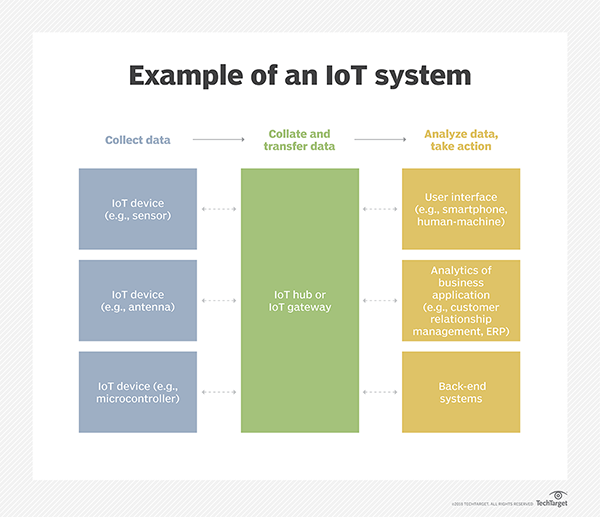
\includegraphics[width=0.7\textwidth]{assets/static/img/iot_system.jpg}
\label{fig:i2c}

\begin{minipage}{0.5\textwidth}
\raggedright \footnotesize Fonte: Retirado de \acite{iot_system} 
\end{minipage}
\end{figure}

\subsection{Evolução da Internet das Coisas}
\hspace*{3em}Na década de 90 a internet foi capaz de facilitar muitos negócios, porém era impactada pela cnexão com velocidade reduzida  e dificuldade no acesso \cite{iot_evolution}. Nos anos 2000 a conectivade com a internet se tornou mais popular de maneira que muitas aplicações passaram a depender desta tecnologia. Com o passar dos anos a dependência da internet se consolidou tornando evidente a necessidade da interação direta do ser humano com dispositivos para gerar resultados e agregar valor, seja para acessar uma página da internet para pesquisas ou realizar negócios em um site de vendas. É nesse contexto que a IoT se insere e permite a conexão das "coisas" para que atividades complexas e que demandam tempo sejam realizadas de maneira dinâmica e automatizada. Tal ideia é mais comum nos dias atuais, pois as residências possuem várias "coisas" com potencial de se comunicar de maneira automatizada. Com o advento da IoT tais "coisas" podem ser controladas facilmente por uma central eletrônica, um navegador de internet ou até mesmo um aplicativo de celular.

\begin{figure}[H]
\centering
\caption{Exemplo de uma casa conectada por um sistema \emph{IoT}}
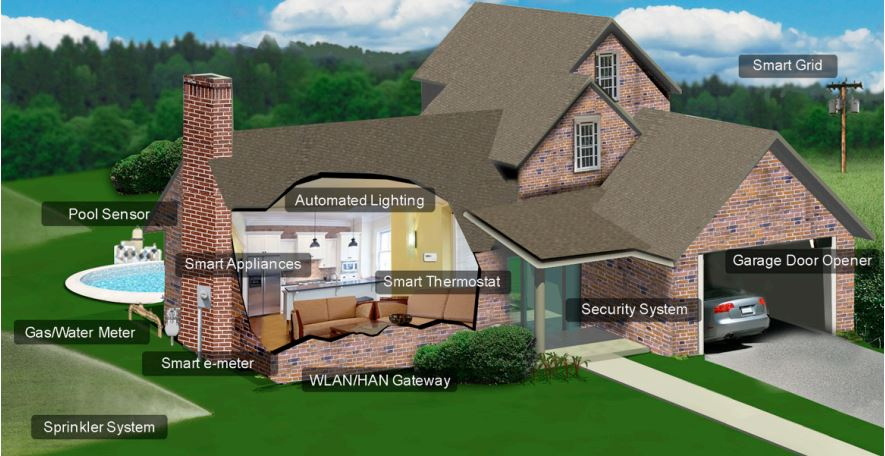
\includegraphics[width=0.7\textwidth]{assets/static/img/iothouse.jpg}
\label{fig:i2c}

\begin{minipage}{0.5\textwidth}
\raggedright \footnotesize Fonte: Retirado de \acite{iothouse} 
\end{minipage}
\end{figure}

\subsection{Indústria 4.0}
\hspace*{3em}A era digital possiblitou a melhora no desempenho de muitos sentores e com isso seu crescimento. A digitalização da manufatura se iniciou na primeira revolução industrial. Naquela época, as máquinas à vapor eram o ápice da tecnologia, estas foram substituídas por motores elétricos durante a segunda revolução. O uso de computadores e equipamentos eletrônicos mais arrojados se estabeleceu somente a partir da terceira revolução industrial e abriu espaço para a indústria 4.0. Nesse cenário, o uso de  computadores com alta capacidade de processamento capazes de automatizar e interligar uma linha completa de sistemas inteligentes emergiu. A inovadora indústria 4.0 tem como cerne o tratamento, processamento e integração dos dados gerados por estes mesmos dispositivos. 
\begin{figure}[H]
\centering
\caption{Revoluções Industriais}
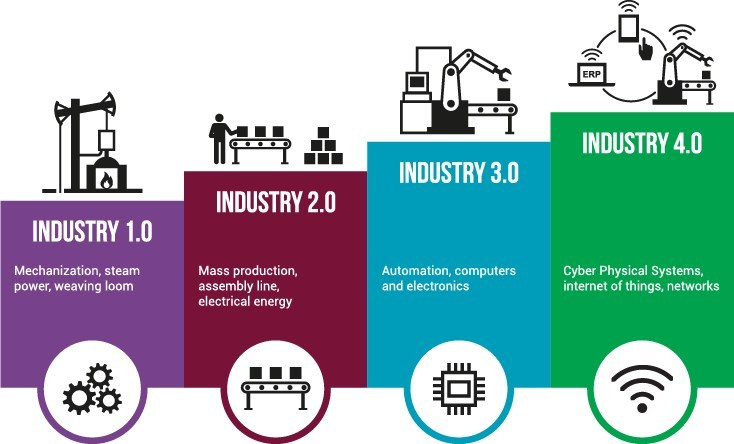
\includegraphics[width=0.5\textwidth]{assets/static/img/ind4.jpg}
\label{fig:i2c}

\begin{minipage}{0.7\textwidth}
\raggedright \footnotesize Fonte: Retirado de \acite{ind4} 
\end{minipage}
\end{figure}


\hspace*{3em}Muitos modelos de tecnologia podem ser abordados para alavancar a Indústria 4.0. Exemplos desses modelos são:
\begin{enumerate}[label=\alph*)]
\itemsep0em
    \item combinações de sistemas ciberfísicos, computacionais colaborativos que controlam entidades ou equipamentos físicos \acite{cyberphysic};
    \item internet das coisas;
    \item aprendizado de máquina (\emph{Machine Learning}).
\end{enumerate}

\hspace*{3em}Os exemplos citados são os meios utilizados para trazer valores para dentro da indústria.  São feitas análises por meio da geração e coleta de inúmeros dados sobre performance, manutenção, rendimento e não-conformidades com o objetivo de identificar oportunidades, otimizar a logística e a sua cadeia de gestão (\emph{Supply Chain}). Robôs inteligentes facilitam a logística de linhas de produção, carros autônomos automatizam o processo e segurança de locomoção e até impressoras 3D atuam independentemente. Com isso, máquinas se tornam autônomas e totalmente independentes da interação humana desde da execução até a finalização do processo. Apesar de parecermos vivenciar essa revolução do começo ao fim, estima-se que a industria 4.0 irá permanecer em evolução durante os próximos 30 anos e que as empresas vão aderir a estas tecnologias aos poucos.

\section{Modelo ultilizado para aplicação}
\hspace*{3em}Para o desenvolvimento da aplicação  utilizamos o modelo cliente servidor, esse modelo permite a modularização da aplicação  em três camadas:  camada de interface com usuário, também conhecida como front-end; camada lógica onde está inserida as regras de negócios, também conhecido como back-end e a camada de dados  onde se realiza a comunicação com o banco de dados. Tal arquitetura permite um desacoplamento de código que viabiliza a atualização das partes de forma independente da tecnologia \cite{3layers}
\section{REST API}
\hspace*{3em}REST (Transferência representacional de estado) API (Interface de programação de aplicação) analisando os conceitos isolados.\par
API é um interface de comunicação disponível por software, com regras estabelecidas para que haja o entendimento de ambas as partes. Esse conceito é aplicado para criar uma camada de abstração, no qual, para utilizar os recursos de um determinado software, é necessário apenas o entendimento da interface disponibilizada, eliminando a  necessidade do entendimento total do aplicação, além de viabilizar o conceito de modularização de arquitetura de software. \cite{16} \par 
REST é um modelo de arquitetura do software criado para suprir conceitos de qualidade e funcionalidade, em princípio, para sistemas distribuídos. Foi utilizada largamente em aplicações WEB.A arquitetura define um conjunto de padrões uniformes para interfaces, sem conservação de estado e separação total do cliente e servidor. Com isso, permite a interoperabilidade entre sistemas. Quando um servidor WEB segue esses conceitos, pode ser denominado REST FULL.\par
Portando uma REST API é uma interface que aplica os conceito REST para sua implementação\cite{19}. Quando o protocolo HTTP é utilizado, o URI (Identificador de recursos uniformes) se torna uma representação dos dados e os métodos HTTP são utilizados para manipular esses dados \cite{16}, com os métodos:

\begin{enumerate}[label=\alph*)]
\itemsep0em
    \item GET para recuperar os dados;
    \item POST para criar novos dados;
    \item PUT para atualizar os dados;
    \item DELETE para apagar os dados.
\end{enumerate}

\section{Backend}
\subsection{Conceito de backend}
\hspace*{3em}Uma aplicação WEB em geral é dividida  em duas principais partes: a camada do \emph{front-end} que é responsável pela interação com o usuário de forma gráfica e o \emph{backend} é responsável por entregar toda a lógica necessária para o front end, geralmente o \emph{backend} é dividido em três elementos responsáveis por implementar a lógica do negócio \cite{16}:

\begin{enumerate}[label=\alph*)]
\itemsep0em
    \item aplicação;
    \item banco de dados;
    \item servidor.
\end{enumerate}

\subsection{Linguagem Backend}
\hspace*{3em}A linguagem mais utilizada para programar dispositivos IoT é a linguagem C pois foi otimizada para essa finalidade, entretanto, por ser uma linguagem de baixo nível, exige uma extensa dedicação de tempo e torna-se morosa para soluções mais complexas. Para contornar essas deficiências, a linguagem Elixir pode ser uma ótima alternativa por ser uma linguagem de alto nível que não compromete a performance do sistema.\par
A linguagem Erlang/Elixir é uma linguagem funcional desenvolvida para atingir alta performance e confiabilidade. Foi desenvolvida para aplicações voltadas para telecomunicações que exigem, baixa tolerância de falhas, distribuida e \emph{real-time} (tempo de execução). Por isso conta com um conjunto bibliotecas para desenvolvimento de sistemas de alta confiabilidade conhecida como OTP.\par
Elixir foi desenvolvida para ser executada na VM (máquina virtual) do Erlang nomeada como BEAM. A linguagem Elixir é relativamente nova, mas já existem diversas aplicações que a utilizam e inclusive existem recursos para dispositivo embarcado como o framework Nerves \cite{ElixirorIoT} e para implementação de aplicações WEB como o framework Phoenix.

\subsection{Nerves}
\hspace*{3em}Nerves é um framework para desenvolvimento de projetos embarcados, baseado em Linux que apenas executa a VM BEAM, portanto proporciona a utilização da linguagem Elixir no desenvolvimento das aplicações. Além disso este framework proporciona diversas vantagens em relação ao processo tradicional de programação de embarcados \cite{nerves}, como:
\begin{enumerate}[label=\alph*)]
\itemsep0em
    \item permitir a fácil portabilidade para diferentes HW (hardware) embarcados e com uma vasta abrangência para diferentes HW embarcados;
    \item fácil manutenção e atualização de firmware por viabilizar a atualizações via OTA (atualização sobre o ar);
    \item dispensa o processo tradicional de dispor do acesso físico, à flash do dispositivo para o armazenamento do firmware;
    \item recursos para facilitar e agilizar o desenvolvimento de firmware;
    \item vasta biblioteca para manipulação dos sistemas embarcados.
\end{enumerate}

\subsection{Phoenix}

\hspace*{3em}Phoenix é um framework desenvolvido em Elixir para implementação de aplicações WEB, que usa todo o potencial da linguagem Elixir, com isso desfruta da concorrência fornecida pela VM BEAM, com baixa tolerância a falha e baixa latência.  Além de aumentar o desempenho do desenvolvimento de uma aplicação WEB também conta com diversos recursos que são disponibilizados de forma modular\cite{phoenix}.

\begin{figure}[H]
\centering
\caption{Diagrama simplificado da arquitetura do software}
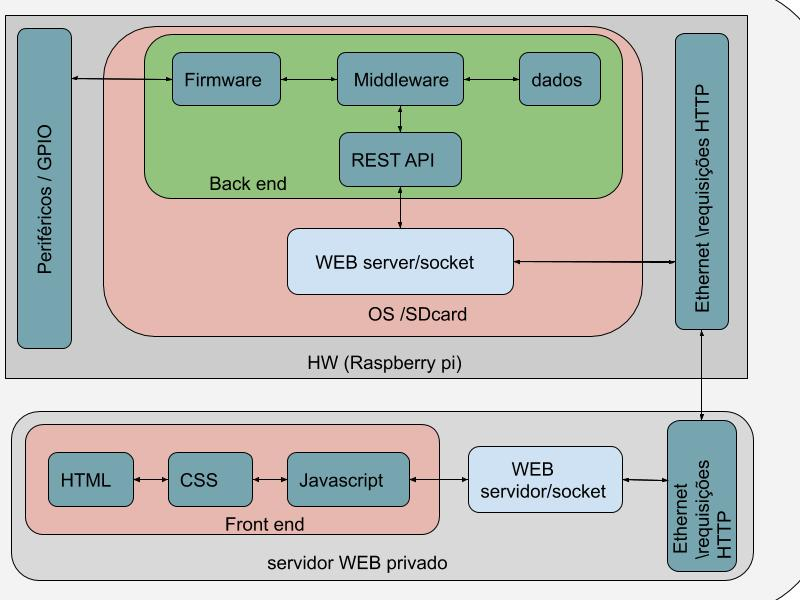
\includegraphics[width=0.5\textwidth]{assets/static/img/diagrama_tcc.jpg}
\label{fig:diagrama_sw}
\end{figure}

\section{Frontend}
\subsection{Conceito de frontend}

\hspace*{3em}Em uma aplicação WEB a camada de front-end é responsável por realizar a interação com usuário, também é conhecida como \emph{client-side} (lado do cliente), pois todos os recursos desenvolvidos são executados em um navegador web alocado em um computador pessoal. Para que essa interface com o usuário seja criada sob demanda, é necessário um fluxo de comunicação entre o \emph{browser} e o servidor. Em geral, o navegador solicita, a partir do protocolo HTTP, uma requisição para o servidor onde estão hospedadas todas as informações visuais necessárias. O backend do servidor recebe essa requisição, realiza as alterações necessárias no servidor e retorna com o conteúdo solicitado. O conteúdo é composto por códigos HTML, CSS e JavaScript, o navegador recebe esse pacote e renderiza de forma visual a informação solicitada. Essas são as três tecnologias essenciais para a construção de uma interface visual web.\cite{frontend}

\subsection{Mobile frontend}
\hspace*{3em}Por  muitos anos o front-end teve como objetivo o navegador para PC, dessa forma os layouts eram desenvolvidos para telas dentro das dimensões padrões dos computadores. Entretanto, com o advento dos dispositivos móveis, foram necessárias adaptações à tecnologia que apesar de muito prematura, já demonstrava importante potencial. Criaram-se então os conceitos de \emph{design} responsivo e \emph{mobile-first} (movél primeiro) que tem como objetivo criar interfaces que podem ser adaptadas para quaisquer que sejam as dimensões das telas, desde um computador até dispositivos como \emph{smartwatch}.\par
Com a tendência de acesso à páginas web a partir de quaisquer dispositivos móveis, houve um realce no potencial da tecnologia IoT, viabilizando o controle de qualquer dispositivo a partir de até mesmo um pequeno \emph{smartwatch} em qualquer lugar do mundo.\cite{mobilefrontend}

\subsection{Hyper Text Markup Language (HTML)}
\hspace*{3em}É uma linguagem de marcação padrão para o desenvolvimento web, que descreve a estrutura de uma \emph{webpage} de forma semântica, por isso é considerada uma linguagem de marcação ao invés de uma linguagem de programação. Essa descrição é renderizada pelo navegador web em uma forma gráfica.\cite{frontend}

\subsection{Cascading Style Sheets (CSS)}
\hspace*{3em}Também é considerada uma linguagem de marcação, porém com o objetivo de criar uma folha de estilo para páginas web. É muito utilizada para modificar a estrutura de uma página web escrita em HTML. O CSS demonstra um aspecto mais moderno com muito mais recursos visuais e de design para as aplicações web. Isso se dá pois o CSS permite alterações no \emph{layout} geral do texto e da página, além de permitir mais agilidade nas aplicações, por diminuir o tamanho dos arquivos em relação ao HTML.\cite{frontend}

\subsection{Javascript}
\hspace*{3em}Javascript é uma linguagem de programação interpretada, multi-paradigma, dinâmica e sem tipos, voltada para desenvolvimento web. Em comparação às linguagens HTML e CSS, que são voltadas para a criação de elementos estáticos na aplicação web, o Javascript permite o desenvolvimento de aplicações mais complexas, trazendo mais dinâmica e versatilidade para as aplicações web.\cite{frontend}

\section{Arquivo JSON e XML}
\hspace*{3em}Para padronizar a transmissão de informações atavés de aplicações e dispositivos diferentes, foram criados vários formatos de texto para sua formatação ideal à aplicação, desenvolvedores e ao próprio usuário. Dessa forma a escolha deve ser analisada para melhor praticidade, desempenho e segurança. O formato JSON (\textit{JavaScript Object Notation}) é utilizado em aplicações compactas, de padrão aberto e de fácil compreensão , sendo muito prática para serem visualizadas de forma geral e escritas ao mesmo tempo, ao contrário de formatações como o XML (\textit{Extensible Markup Language}), o JSON é uma formatação totalmente independente que surgiu do JavaScript, porém usa convensões familiares de outras linguagens da família C (C, C++, C#), Python, Pearl, o que a torna muito prática para formatação em várias plataformas. A seguir, exemplos da formatação em XML e JSON:

\begin{enumerate}[label=\alph*)]
\itemsep0em
  \item XML:
    \begin{minted}[xleftmargin=\parindent,tabsize=2,breaklines]{xml}
<?xml version="1.0" encoding="UTF-8"?>
<cardapio>
<comida>
    <nome>Hot Dog</nome>
    <preco>R$ 8,99</preco>
    <descricao>
   	Pão com salsicha completo (acompanha batata palha, ketchup e maionese)
   	</descricao>
    <calorias>650</calorias>
</comida>
<comida>
    <nome>Hamburguer</nome>
    <preco>R$ 10,99</preco>
    <descricao>
    Pão com 1 fatia de hambúrguer, 3 fatias de tomate, salada, ketchup e 1 fatia de queijo
    </descricao>
    <calorias>950</calorias>
</comida>
</cardapio>
    \end{minted}
  
  \item JSON:
    \begin{minted}[xleftmargin=\parindent,tabsize=2,breaklines]{js}
[
   {
      "nome": "Hot Dog",
      "preco": "R$ 8,99",
      "descricao": "Pão com salsicha completo (acompanha batata palha, ketchup e maionese)",
      "calorias": "650"
   },
   {
      "nome": "Hamburguer",
      "preco": "R$ 10,99",
      "descricao": "Pão com 1 fatia de hambúrguer, 3 fatias de tomate, salada, ketchup e 1 fatia de queijo",
      "calorias": "950"
   }
]
    \end{minted}
\end{enumerate}

O formato JSON, como mencionado, tem um visual mais limpo, com uma leitura mais simples do arquivo e maior velocidade na manipulação e transmissão dos dados.

\section{Segurança em software}
\hspace*{3em}Com o crescimento da tecnologia \emph{IoT} nasceram novos problemas de segurança, uma vez que existe uma grande diversidade e quantidade de objetos conectados na rede. O principal problema se dá pela falta de cuidado no design de software o que abre caminho para que \emph{malwares} e \emph{backdoors} se instalem. Além disso, identificar a localização dos objetos na rede e gerar métodos de autenticação seguros (métodos tradicionais não são aplicáveis devido a heterogeneidade dos objetos) são importantes problemas a serem solucionados. Outro obstáculo está em manter a privacidade dos dispositivos \emph{IoT}. Durante o uso da tecnologia, dados do comportamento e da rotina diária são coletados a fim de melhorar os serviços e a experiência pessoal de cada usuário. Entretanto, as informações coletadas descrevem o usuário detalhadamente, portanto é necessário cautela quanto à exposição desses dados, para evitar o uso indevido de informações pessoais. 
É importante ainda ter em mente que alguns dispositivos possuem capacidade computacional limitada e restrições de consumo elétricos, por terem baterias menos robustas, por tanto não suportam  sistemas complexos de criptografia. Estes sistemas exigem poder computacional elevado e consequentemente elevado consumo de energia, devido à isso é importante diversificar a criptografia para assegurar maior privacidade ao usuário. Algoritmos mais simplificados de criptografia são mais adequados para dispositivos com restrição de recursos. Uma segunda solução é ocultar alguns dados, porém isso ainda é um obstáculo uma vez que os objetos conectados precisam ter acesso a tais informações. \cite{seguranca}

\section{Protocolos de comunicação}
\end{document}
